\documentclass[10pt,twocolumn,letterpaper]{article}
\usepackage[final]{cvpr}
\usepackage{graphicx}
\usepackage{booktabs}
\usepackage{amsmath,amssymb}
\usepackage{multirow}
\usepackage{xcolor}
\usepackage{url}
\usepackage{microtype}
\graphicspath{{figures/}}

\definecolor{cvprblue}{rgb}{0.21,0.49,0.74}
\usepackage[pagebackref,breaklinks,colorlinks,allcolors=cvprblue]{hyperref}
\def\paperID{internal}
\def\confName{Internal Review}
\def\confYear{2026}
\title{When Agreement Hides Error:\\
Auditing Shared Measurement Dependence in MRI Slice Interpolation}
\author{Internal scientific review draft}
\begin{document}
\maketitle
\noindent\textbf{Internal scientific review draft (2026-10-01).} Not a submission version; data-use and ethics documentation remain unresolved.\par\smallskip

\begin{abstract}
Agreement between MRI reconstructions can conceal error when they reuse observed slices. We audit this failure in retrospective through-plane T2 interpolation by holding the target and a frozen reference prediction fixed while changing the real-slice context supplied to a companion estimator. Across the previously studied fastMRI and IXI cohorts, disjoint contexts increased the fraction of paired-error energy visible in disagreement in all 20 ordered cross-architecture comparisons per cohort. A protocol-frozen HAT-to-SwinIR pair showed a patient-weighted disjoint-minus-shared observability difference of 19.76 percentage points (95\% patient-bootstrap interval, 19.33--20.16) in 84 separately sourced MSValid RRMS patients. A later frozen IXI-weight pair showed 26.40 points (stratified interval, 25.69--27.17) in 62 TCIA ReMIND preoperative brain-tumor patients. Earlier acquired-only response analyses supported conditional error-alignment associations, but a 60-patient heldout test found no prediction gain from continuous response influence beyond an exact-context baseline. These interventions change companion context, geometry and potentially normalization; ReMIND's published DICOMs also carry an MPR flag. This is a bounded audit of shared measurement dependence, not a causal identity estimate, calibrated per-case detector or test of true thin-slice recovery.
\end{abstract}

\section{Introduction}
Prediction agreement is often treated as evidence of reliability. It is more informative when alternative predictions fail differently and less informative when they inherit the same error. Our question is: \emph{when does prediction agreement cease to be evidence of reliability?} We study deterministic cross-context disagreement, not all Bayesian, probabilistic, or calibrated uncertainty methods.

MRI slice interpolation offers a controlled setting for this question. A retrospectively available dense examination identifies the missing target plane, the acquired slice positions, and the physical identity of each anchor. Two contexts can reconstruct the same target while sharing or separating acquired measurements. This lets us intervene on evidence dependence rather than merely compare networks with different architectures or accuracy.

\begin{figure*}[t]
\centering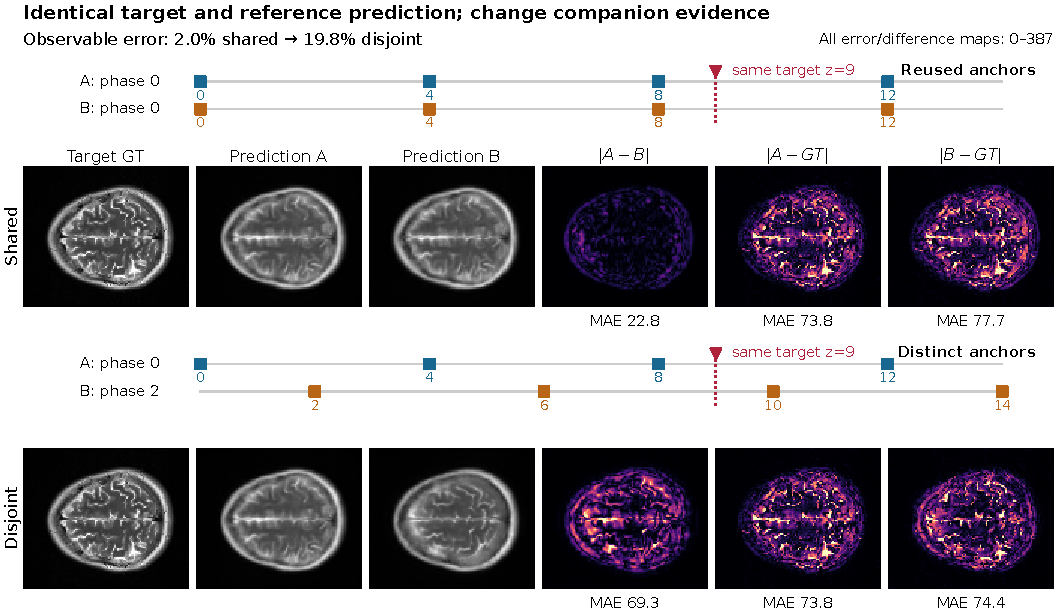
\includegraphics[width=.98\textwidth]{final_fig1_physical_anchors.pdf}
\caption{Shared measurements can conceal aligned error. A fixed median-effect fastMRI example uses frozen SwinIR weights. Physical anchor strips identify reused and distinct measurements; the target and prediction A are identical across rows. Shared inputs give small disagreement despite substantial error. Disjoint inputs expose more of that error. All error and disagreement maps share one scale. The supplement gives the fixed selection rule, precision check and a seeded random example.}
\label{fig:teaser}
\end{figure*}

Figure~\ref{fig:teaser} shows the failure directly. Under shared anchors, the two predictions smooth the same structures and largely agree on their errors. Disjoint anchors need not make either reconstruction substantially more accurate; they change which error components become visible in the difference. The distinction matters: low disagreement is an observation about two outputs, not a certificate about their unknown target.

The error-difference identity is elementary, and variability missing systematic MRI error is already known~\cite{hu2021predict}. Our contribution is an executable \emph{Measurement-Influence Reliability Audit} (MIRA). It specifies the physical intervention, quantities that require ground truth, local influence computation, stability checks, and unit of statistical inference. A local covariance model explains why shared anchors matter through estimator sensitivity rather than through their count alone. Controlled experiments then test where this explanation succeeds and where it fails.

The distinction between local geometry and global utility is central. A repeatable reduction in observable error does not imply that disjoint disagreement always ranks examinations better. Nor does a stable finite-response probe establish a universal scalar score. We distinguish evidence for a conditional mechanism from evidence for useful error ranking, and retain the failures of attempted scalar scores.

Our contributions are: (1) a same-target audit of local observability loss across diverse frozen estimators and one protocol-frozen, separately sourced single-pair confirmation; (2) a conditional finite-response account of shared influence, accompanied by a strict external prediction failure; and (3) an evidence hierarchy that retains incompatible interfaces, historical stability failures and null results. The project is retrospective, with cohort reuse documented below.

\section{Related Work}
\paragraph{Diversity, covariance and uncertainty.}
The interaction between ensemble error and diversity is established by ambiguity decompositions, negative-correlation learning and diversity measures~\cite{krogh1994ensembles,liu1999negative,kuncheva2003diversity,brown2005diversity,ortega2022diversity}. Random-subspace methods and gradient-diversity training already diversify inputs or sensitivities~\cite{ho1998subspace,kariyappa2019diversity}. We do not claim a new error identity or that diversity first becomes meaningful through MIRA. Our distinction is a controlled physical-measurement intervention with frozen, possibly different estimators, a response audit and explicit failure boundaries.

\paragraph{MRI uncertainty and practical reliability.}
Deep ensembles, dropout, TTA and posterior reconstruction characterize predictive variation~\cite{lakshminarayanan2017ensembles,gal2016dropout,wang2019tta,edupuganti2021uncertainty,narnhofer2022bayesian,luo2023diffusion}. Hu \etal distinguish random and systematic MRI error~\cite{hu2021predict}; common-error blindness is not new. Unlike a posterior sampler, MIRA tests how measurement identity and local responses affect the interpretation of deterministic agreement. Error/OOD detection and selective prediction evaluate actionable ranking or abstention~\cite{hendrycks2017baseline,geifman2017selective}. Our local energy result does not establish those downstream properties, and the scoring failures remain relevant.
Supervised pixelwise MRI error intervals and decompositions of inverse-problem ambiguity address related but different targets~\cite{giannakopoulos2026pixelwise,guo2026ambiguity}. We do not claim the first MRI error map, calibrated interval, or decomposition of intrinsic uncertainty. Our distinction is the fixed-predictor, same-target real-slice context intervention and its bounded paired-error audit.

\paragraph{Consistency and interpolation.}
Acquired-data consistency~\cite{lustig2010spirit} differs from agreement between two missing-slice estimates. We audit HAT/SwinIR and frozen I3Net, SAINT-style and CycleINR-style implementations~\cite{chen2023hat,liang2021swinir,song2024i3net,peng2020saint,fang2024cycleinr}, without proposing an interpolator. Complementary acquisitions and high-order slice interpolation are established~\cite{greenspan2002interslice,nicastro2022shift,horvath2017highorder}. The question here is when agreement hides error, not whether complementary slices or interpolation holdouts are new.

\section{Our Measurement-Influence Framework}
\subsection{Error observability}
Let $F_a,F_b$ be frozen reconstruction estimators (possibly identical) and $c_a,c_b$ two contexts for target location $z$. On a common support, predictions $f_a,f_b$ have errors $e_a=f_a-y$ and $e_b=f_b-y$. The observable is $D=\|f_a-f_b\|$; the target $y$ is unavailable when forming a deployment score. Retrospectively,
\begin{equation}
D^2=\|e_a\|^2+\|e_b\|^2-2\langle e_a,e_b\rangle .\label{eq:difference}
\end{equation}
Define $T=(\|e_a\|^2+\|e_b\|^2)/2$, common error $\bar e=(e_a+e_b)/2$, and difference error $h=(e_a-e_b)/2$. For $T>0$,
\begin{equation}
S=\|\bar e\|^2/T,\quad O=\|h\|^2/T,\quad S+O=1.\label{eq:energy}
\end{equation}
These are latent evaluation quantities, not estimated probabilities. If $e_a=e_b\ne0$, then $O=D=0$ despite error. Conversely, $\max(\|e_a\|,\|e_b\|)\ge D/2$ gives only a one-sided error bound. Shared fractions and normalized disagreement are algebraically related; their correlation is not independent evidence for a mechanism.

\subsection{Controlled same-target measurement intervention}
The framework takes frozen $F_a,F_b$, target location $z$, two target-preserving contexts, and a registry of physical anchor identities. It records model weights, preprocessing, score support, target geometry, and information used to define each. The intervention holds the target and estimator identities fixed while varying anchor identity; relevant geometry is matched where feasible and remaining differences are reported.

At $\times4$, phase-0 anchors $\{0,4,8,\ldots\}$ and phase-2 anchors $\{2,6,10,\ldots\}$ are disjoint. Targets with residues 1 or 3 are absent from both. A shared control applies an in-plane flip to the same phase-0 anchors, then maps predictions back. This is a deterministic test-time augmentation (TTA) pair. A disjoint pair instead compares phase-0 and phase-2 reconstructions. It changes measurement dependence together with the companion context; it is not an intervention that fixes every nuisance variable. Nearest-anchor distances can be matched as the multiset $\{1,3\}$ up to reflection, but full signed geometry and context normalization may still differ. The cross-architecture experiment instead compares $A_0/B_0$ with the identical $A_0/B_2$, without a flip or other TTA. This directly tests whether the phenomenon extends beyond same-network equivariance.

\begin{figure}[t]
\centering
\begin{minipage}{.97\columnwidth}
\hrule\smallskip
\textbf{Algorithm 1: Measurement-Influence Reliability Audit}\par
\smallskip\small
\textbf{Input:} frozen $F_a,F_b$; target locations; anchor-ID registry; declared contexts, preprocessing, support, and perturbation settings. Retrospective targets are a separate evaluation input.\par
\textbf{1. Validate} same-target mapping, acquired IDs, model weights, geometry, and source of masks/scales.\par
\textbf{2. Reconstruct} shared and disjoint pairs; store $f_a,f_b$ and their disagreement on the same support.\par
\textbf{3. Estimate influence} from embedded coefficients or matched anchor responses using Eq.~\ref{eq:influence}.\par
\textbf{4. Check stability} across declared amplitudes/signs; retain failed models as phenomenon-only evidence.\par
\textbf{5. Evaluate retrospectively} alignment, $S,O$, and error ranking; aggregate and resample whole examinations/patients.\par
\textbf{6. Report} all eligible contrasts, uncertainty, failures, and the information-access boundary.\par
\textbf{Output report card:} (i) local observability gap; (ii) named examination-ranking gap; (iii) beyond-count advantage; (iv) fixed-count association; (v) stability PASS/FAIL/NA; (vi) information contract; (vii) claim eligibility. Unmeasured fields remain NA; no combined scalar.\par
\smallskip\hrule
\end{minipage}
\end{figure}

\subsection{Analytical shared influence and a local model}
For $f_c=\sum_j w_{cj}x_j$, embed coefficients in the union of physical anchor IDs, assigning zero to unused anchors. Under independent anchor perturbations with variances $\sigma_j^2$, the shared contribution to output covariance is proportional to $\sum_{j\in c_a\cap c_b}w_{aj}w_{bj}\sigma_j^2$. Overlap count discards sign, magnitude, and noise covariance. Coefficient cosine and common absolute mass $\sum_j\min(|w_{aj}|,|w_{bj}|)$ are descriptive alternatives; common mass alone does not prove positive covariance when coefficients have opposite signs.

\paragraph{Proposition 1 (shared variation under fixed marginals).}
Condition on a fixed target and nominal inputs. Assume the local error model
\begin{equation}
e_a=b_a+J_a\xi_a,\qquad e_b=b_b+J_b\xi_b,\label{eq:local}
\end{equation}
with fixed biases/Jacobians, zero-mean perturbations, marginal covariances $\Sigma_a,\Sigma_b$, and cross-covariance $C=\mathbb E[\xi_a\xi_b^\top]$. Compared with $C=0$ at unchanged marginals and biases, let $\kappa=\operatorname{tr}(J_a C J_b^\top)$. Then
\begin{align}
\Delta\mathbb E\langle e_a,e_b\rangle&=\kappa,\\
\Delta\mathbb E\|f_a-f_b\|^2&=-2\kappa.\label{eq:covariance}
\end{align}
If $\tau=\mathbb E T>0$, the ratio-of-expectations observable fraction $\widetilde O=\mathbb E\|h\|^2/\tau$ changes by $-\kappa/(2\tau)$. Thus positive shared sensitivity increases the expected error inner product and suppresses disagreement energy. Shared variation with opposing sensitivities can do the reverse.

\emph{Proof sketch.} Expanding Eq.~\ref{eq:local}, zero means remove the bias--noise cross terms, leaving $\langle b_a,b_b\rangle+\operatorname{tr}(J_a C J_b^\top)$. Marginal error energies do not depend on $C$; substitute into Eq.~\ref{eq:difference}. The supplement gives the full derivation, remainder qualification, and numerical checks.

This proposition is conditional and local. It does not prove that sharing creates common deterministic bias, that error-vector cosine increases in every realization, or that $\mathbb E O=\widetilde O$. Actual phase interventions can change biases and Jacobians. Their effect therefore requires empirical testing rather than following automatically from the proposition.

\subsection{Neural finite-response shared influence}
For anchor $j$ and a matched zero-mean field $\xi_{js}$, compute $r_{cjs}=F_c(x+\epsilon\xi_{js})-F_c(x)$; absent anchors have zero response. The implemented statistic is
\begin{equation}
\widehat I=
\frac{\sum_s\sum_{j\in c_a\cap c_b}\langle r_{ajs},r_{bjs}\rangle}
{\sqrt{\bigl(\sum_s\sum_{j\in c_a}\|r_{ajs}\|^2\bigr)
\bigl(\sum_s\sum_{j\in c_b}\|r_{bjs}\|^2\bigr)}}.\label{eq:influence}
\end{equation}
It is the cosine of response vectors embedded in physical-anchor space, \emph{not} the average cosine of individual shared-anchor responses. Its denominator includes unshared-anchor energy. Under a local linear response and independent matched anchor fields of covariance $\Sigma_j$, the expected numerator, divided by the number of fields and $\epsilon^2$, is $\sum_j\operatorname{tr}(J_{aj}\Sigma_jJ_{bj}^\top)$, the shared covariance term. The normalized finite-sample ratio is a directional proxy, not an unbiased covariance estimator.

We use four centered Rademacher fields, primary amplitude .01 and alternatives .005/.02/$-.01$. Clipping is part of the finite response. The new acquired-only experiment fixes its mask and Q99--Q1 scale from acquired slices before responses, then accesses targets only for evaluation. FP32 without AMP/TF32 is fixed in its protocol. Historical full-examination scales and target-derived masks remain a different contract. HAT/SwinIR retain their per-stratum .85 rank-stability criterion; SAINT-style uses the separate frozen new-architecture .90 gate. Passing a numerical gate does not establish global Jacobian accuracy.

\subsection{Reliability interpretation and scope}
Algorithm 1 requires no estimator retraining. With retrospective targets it can expose how much common error agreement conceals and whether influence explains variation beyond count. Without targets it can measure disagreement, anchor sharing, and suitably defined local response, but it cannot identify an arbitrary common bias. The framework is therefore an audit, not a calibrated detector of every individual failure. Reused test cohorts and outcome-informed analysis choices are explicitly part of its evidence record.

\section{Experimental Design and Provenance}
\paragraph{Cohorts and frozen implementations.}
We use 24 locally catalogued NYU fastMRI brain T2 examinations~\cite{knoll2020fastmri,muckley2021brain,fastmri_portal}, 115 IXI brain T2 examinations~\cite{ixi_dataset}, and 22 NingXia knee T2 series from eight patients. Existing dataset-specific training splits or patient-group out-of-fold models supply the weights. HAT/SwinIR cover all three cohorts; locally configured I3Net, adapted SAINT-style and internal CycleINR-style add three brain-cohort lineages. These are frozen local implementations, not claims of exact official reproductions. Wrapper verification and the declared SAINT coordinate correction are detailed in the supplement.
The separately sourced public MSValid RRMS brain T2 cohort~\cite{msvalid2024zenodo} supplies an additional single-pair confirmation. After inspecting it, we froze a further source-specific single-pair test on TCIA ReMIND preoperative brain-tumor T2 DICOMs~\cite{remind_tcia}. Neither is part of the old 20-pair matrix. Data rights for locally held fastMRI material and the NingXia source, de-identification, ethics and consent records require author verification before submission.

\paragraph{Primary analyses and bounded coverage closure.}
(1) All 20 ordered cross-architecture pairs per brain cohort use five missing planes per examination and one identical target-derived 1\% mask. The fixed reference $A_0$ is unchanged. (2) Acquired-only influence uses both HAT/SwinIR, three depth-selected targets, reference $(-2,+2)$ and eight non-self contexts from offsets $\{\pm1,\pm2,\pm3\}$. Four contexts share exactly one anchor. A six-plane acquired pool defines a common scale; the nearest acquired foreground union defines support. (3) Twelve hash-selected IXI examinations test coupled versus independent perturbations at fixed nominal contexts, both models and all four one-anchor comparators. The supplement gives complete geometry, precision and noise settings. The bounded closure repeats (2) for SAINT-style and, conditional on numerical stability, (3). I3Net/CycleINR cannot consume the exact two-anchor variable-spacing probe without changing their frozen four-anchor contract. They retain NA for acquired-only influence, separately from historical stability failures. No score or threshold is searched.

\paragraph{Statistical units and study status.}
Examinations are independent units; NingXia resamples patients with all subordinate observations. New cross-architecture points average five planes within each examination, then average examinations. Ranking correlates examination means. New influence points pool planes/contexts, with examination bootstrap and fixed-count geometry/examination adjustment. Simultaneous 95\% intervals use 5,000 paired examination draws and maximum standardized deviation: 20 ordered pairs per cohort/endpoint, two models per influence cohort/endpoint, or eight model/amplitude contrasts. Original pooled-plane controls and historical five-model inference remain separately labeled. Their families are unchanged: new SAINT influence intervals cover both cohorts per endpoint, and its covariance intervals cover four amplitudes. These extension families do not claim joint coverage across the old and new studies.

The final protocol, inputs, masks, checkpoints and case/pair registries were frozen before new inference. This is a frozen retrospective iteration, not preregistration or an untouched holdout. Earlier outcomes informed the project; some historical controls and endpoints evolved. Local IDs show one fastMRI training/validation patient overlap but no test overlap, disjoint IXI IDs and patient-group NingXia folds. Selection uncertainty across the research history is outside the reported bootstrap intervals. Full provenance, unresolved release/ethics documentation and negative results are in the supplement. The present support and geometry checks are post-hoc sensitivities, separately frozen before calculation; they do not change the primary protocol.
\paragraph{Separately sourced MSValid confirmation.}
Before accessing missing target pixels, we fixed the first available T2 volume per patient, 84 geometry-qualified examinations and 479 residue-1/3 targets, the fastMRI-trained HAT and SwinIR checkpoints, CPU FP32 inference, an acquired-only foreground support, and patient-level inference. Native z spacing was 3--6 mm. HAT retained phase-0 real-slice anchors; SwinIR used either the same phase-0 anchors or a disjoint phase-2 real-slice context to reconstruct the identical withheld native plane. Both conditions used observed-only normalization. The primary endpoint was the patient-weighted disjoint-minus-shared difference in $O$, averaging the two target residues equally within each patient. Its prespecified interval used 5,000 paired patient-bootstrap draws. The native thick-slice scans were retrospectively subsampled $\times4$; this is not a test of independently acquired thin-slice recovery. Source-file, checkpoint, script and protocol hashes and wrapper-equivalence checks are retained in the audit archive. These MSValid data and its single-pair interval are separate from all original inference families.

\paragraph{Later ReMIND source confirmation.}
Before decoding ReMIND pixels, we fixed all 63 official preoperative 2D axial T2/T2 BLADE series (one per patient), DICOM-header eligibility, IXI-trained HAT/SwinIR checkpoints, four residue-1/3 targets per eligible patient, acquired-only support, CPU FP32 inference and the same fixed-reference phase intervention. One 21-slice series failed the prespecified 24-slice header threshold; the other 62 patients contributed 248 targets. The primary patient-weighted $\Delta O$ used 5,000 stratified patient-bootstrap draws, preserving the 35 ordinary-T2 and 27 BLADE patients; both stratum point estimates had to be positive, along with a positive pooled interval lower bound and prespecified completion counts. The protocol was designed after the MSValid result, but before ReMIND target pixels were read. Published ReMIND DICOMs carry an MPR image-type flag, so physical layer independence cannot be inferred from these headers.

\paragraph{Model-evidence accounting.}
The bank contains 13 reconstruction implementations and 111 recorded configurations. Table~\ref{tab:coverage} separates reconstruction, phase intervention, acquired-only influence and covariance evidence. The additional eight baseline phase tests are secondary architecture-breadth sensitivities with an exact-repeat shared control, whose zero disagreement is constructed. They establish interface and phase-response coverage, not eight independent validations of the shared-error mechanism. The five-architecture cross-model matrix remains primary.
\begin{table*}[t]\centering\footnotesize
\caption{Model--evidence coverage. $\checkmark$: supported within the named design; $\circ$: evaluated but null/inconclusive; $\times$: numerical or interface eligibility failed; --: not run/not applicable. Subscript $s$: secondary exact-output-repeat control, so shared $O=0$ is constructed, not independent mechanism evidence. Subscript $a$: interface audit only; see the current full-bank table for evaluated continuous influence. $\times_h$: historical target-informed stability failure; current acquired-only stability is NA. Current cohort-specific effects and numerical gates are in Table~\ref{tab:continuous-big}; historical SAINT null evidence remains in the supplement. Covariance coverage is unchanged. Native reconstruction metrics remain in the supplement.}
\label{tab:coverage}\setlength{\tabcolsep}{3pt}
\begin{tabular}{lcccccll}\toprule
Model & Recon. & Same-model & Cross-arch. & Acq. influence & Stability & Covariance & Role in claims\\\midrule
Linear & $\checkmark$ & $\checkmark_s$ & -- & $\checkmark$ & $\checkmark$ & -- & Phase; influence in large table \\
Cubic & $\checkmark$ & $\checkmark_s$ & -- & $\times$ & -- & -- & Secondary phase sensitivity \\
ACVTT & $\checkmark$ & $\checkmark_s$ & -- & $\times$ & $\times$ & -- & Phase; influence in large table \\
Res-SRDiff & $\checkmark$ & $\checkmark_s$ & -- & $\times$ & -- & -- & Secondary phase sensitivity \\
ArSSR & $\checkmark$ & $\checkmark_s$ & -- & $\checkmark$ & $\checkmark$ & -- & Phase; influence in large table \\
CycleINR-style & $\checkmark$ & $\checkmark$ & $\checkmark$ & $\times$ & NA [$\times_h$] & -- & Phenomenon; probe ineligible \\
ResUNet & $\checkmark$ & $\checkmark_s$ & -- & $\checkmark$ & $\checkmark$ & -- & Phase; influence in large table \\
Pix2Pix-GAN & $\checkmark$ & $\checkmark_s$ & -- & $\times$ & -- & -- & Secondary phase sensitivity \\
SwinIR & $\checkmark$ & $\checkmark$ & $\checkmark$ & $\checkmark$ & $\checkmark$ & $\checkmark$ & Phenomenon + local influence \\
SAINT-style & $\checkmark$ & $\checkmark$ & $\checkmark$ & $\checkmark\,[\circ_h]$ & $\checkmark$ & $\checkmark$ & Phenomenon + local influence \\
I3Net & $\checkmark$ & $\checkmark$ & $\checkmark$ & $\times$ & NA [$\times_h$] & -- & Phenomenon; probe ineligible \\
HAT & $\checkmark$ & $\checkmark$ & $\checkmark$ & $\checkmark$ & $\checkmark$ & $\checkmark$ & Phenomenon + local influence \\
SMamba-UNet & $\checkmark$ & $\checkmark_s$ & -- & $\checkmark$ & $\checkmark$ & -- & Phase; influence in large table \\\bottomrule\end{tabular}\end{table*}

\section{Results}
\subsection{Protocol-frozen confirmation on a new source}
All 84 MSValid patients and 479 qualified targets were scored without failure. Patient-weighted $O$ rose from 2.8428\% with shared anchors to 22.5993\% with disjoint anchors, a 19.7565 percentage-point difference (95\% patient-bootstrap interval 19.3276--20.1605); all 84 patient differences were positive. The companion SwinIR patient-weighted MAE was 141.68 under sharing and 139.06 under disjoint context in within-volume raw intensity units. Thus the primary gap does not simply reflect higher average companion MAE. Exploratory phase reversal, a linear companion, and common six-anchor min/max normalization retained disjoint-minus-shared differences of 19.50, 14.62, and 19.48 points. These post-result controls are sensitivity checks, not independent confirmations. An algebraic decomposition of the same endpoint assigned approximately 0.15 points to companion MSE imbalance and 19.61 points to the paired-error alignment term; it adds no independent causal evidence.

\paragraph{Secondary IXI-weight pair on the same patients.}
After inspecting the primary result, we froze a second HAT-to-SwinIR contrast using IXI-T2-trained checkpoints and the same 84 MSValid patients, 479 targets and scoring contract. Patient-weighted $O$ rose from 1.0420\% to 25.2276\%: disjoint minus shared was 24.1856 percentage points (exploratory 95\% patient-bootstrap interval 23.7150--24.6726), positive in all 84 patients. Companion MAE was 130.33 under sharing and 129.46 under disjoint context. This broadens frozen-weight-pair coverage on a public-data training source, but does not add an independent cohort or a second prespecified external confirmation.

\paragraph{ReMIND preoperative T2 source.}
All 62 header-eligible patients and 248 fixed targets completed CPU inference; the sole exclusion was the predeclared short series. Shared and disjoint patient-weighted $O$ were 1.1093\% and 27.5092\%, a $\Delta O$ of 26.3999 percentage points (95\% stratified patient-bootstrap interval 25.6945--27.1686). All 62 patient differences were positive. Ordinary T2 and BLADE estimates were 26.5156 and 26.2500 points, meeting both prespecified stratum-direction checks. Companion MAE was 132.13 with shared and 131.71 with disjoint context in within-scan intensity units. A separate read-only audit verified source ZIP hashes, fixed targets, per-target energy identities, patient aggregation and the seeded interval. This is a different patient source, not independent discovery of the test design or replication of the full architecture matrix.

\subsection{Phenomenon: common error becomes invisible}
Figure~\ref{fig:control} and Table~\ref{tab:controlled} re-express the original two-architecture clean comparison using one local estimand: the fraction of paired-error energy visible in disagreement. Shared and disjoint conditions use identical paired targets and the original prediction-derived support. Examinations/patients and models receive equal weight; series are first averaged within NingXia patients. Shared $O$ is small in every cohort, while disjoint evidence exposes more error. Historical pooled-plane ranking and stable-wrong prevalence remain in the supplement, with their original endpoints and aggregation. This descriptive re-expression does not create a new confirmatory experiment.

\begin{table}[t]\centering\small
\caption{Original clean same-model control, re-expressed with uniform local estimands. Target means, equal model means and patient/examination means; NingXia first averages series within patient. Pointwise 95\% paired cluster intervals. $O$ is in percent; $\Delta O$ in percentage points.}
\label{tab:controlled}\setlength{\tabcolsep}{3pt}
\begin{tabular}{lrrrr}\toprule Cohort & Units & Shared $O$ & Disjoint $O$ & $\Delta O$ [CI]\\\midrule
fastMRI & 24 & 2.61 & 19.35 & 16.74 [15.73,17.74] \\
IXI & 115 & 1.58 & 30.21 & 28.63 [28.19,29.07] \\
NingXia & 8 & 0.25 & 15.28 & 15.03 [13.73,16.35] \\\bottomrule\end{tabular}\end{table}
\begin{figure*}[t]
\centering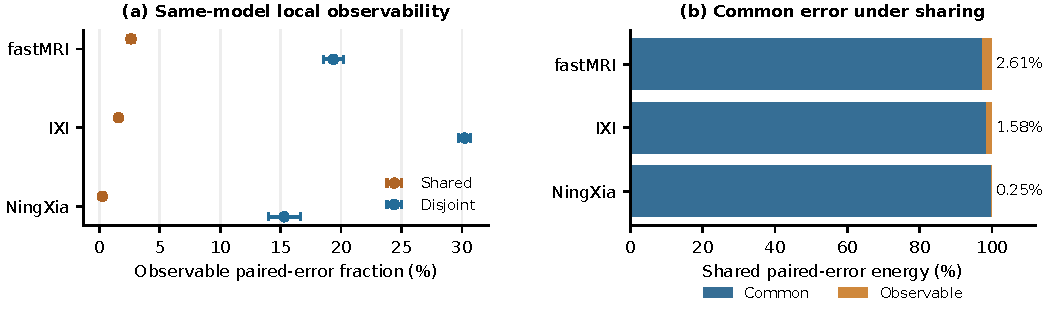
\includegraphics[width=.95\textwidth]{final_fig2_original_control.pdf}
\caption{Local error observability in the original clean same-model experiment. (a) Shared/disjoint observable fractions, with pointwise 95\% patient/examination-bootstrap intervals. (b) Common versus observable energy under sharing, using the same observations and aggregation. Target planes, models and subordinate series are averaged before the independent unit. The energy decomposition is descriptive, not independent evidence for its own algebraic identity.}
\label{fig:control}
\end{figure*}

The objectively selected example in Fig.~\ref{fig:teaser} makes the spatial failure visible. Shared prediction MAEs are 73.8 and 77.7 but their difference MAE is 22.8; observable fraction is 2.0\%. With the same target and reference prediction, disjoint difference MAE rises to 69.3 and observable fraction to 19.8\%, while paired error changes little. These values describe that example, not an estimate of prevalence. Its CPU predictions differ slightly from historical mixed-precision outputs; the cohort statistics are unchanged.

\subsection{Mechanism: acquired-only influence beyond count}
Overlap count is not a monotone dose: the analytical ladder reverses from zero to one shared anchor in every original cohort. The new acquired-only probe asks whether continuous response influence retains information when neither its scale nor support accesses the missing target. On IXI, beyond-count alignment advantages are .098/.093 for HAT/SwinIR; on fastMRI they are .103/.093. Every original two-model simultaneous interval is positive (Fig.~\ref{fig:influence}, Table~\ref{tab:continuous-big}). At exactly one shared anchor, partial associations adjusting span, asymmetry and examination are .270/.265 on IXI and .474/.365 on fastMRI, again with positive simultaneous intervals.

\begin{figure*}[t]
\centering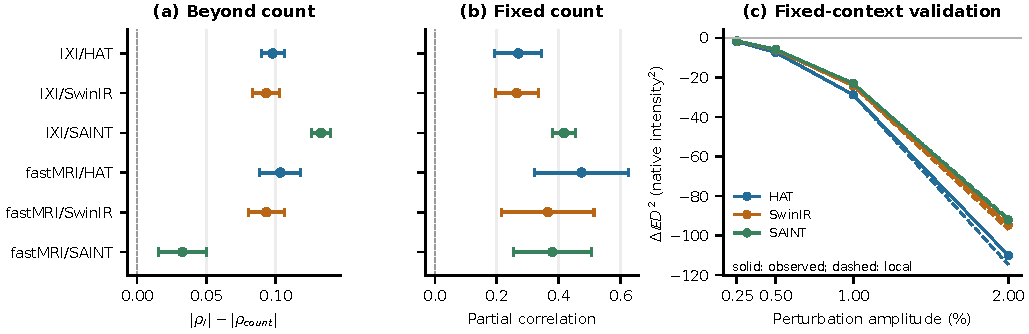
\includegraphics[width=.98\textwidth]{final_fig3_acquired_influence.pdf}
\caption{Earlier three-model experiments with acquired-only masks and scales; their original inference families are retained here. The new full-bank comparison is in Table~\ref{tab:continuous-big}. (a) Absolute alignment-correlation advantage over count. (b) Exactly-one-anchor partial correlation adjusting geometry and examination. HAT/SwinIR intervals retain the original two-model family per cohort/endpoint; the new SAINT family covers both cohorts per endpoint. Targets enter only error evaluation. (c) Signed coupled-minus-independent disagreement-energy change and the fixed $\epsilon_0=.0025$ prediction for all three models and four amplitudes. Aggregate trends agree; original HAT/SwinIR median individual relative errors are 1.9--10.6\%, but the worst individual error is 126.4\%: there is no uniform Jacobian guarantee. Complete individual scatter is retained in the supplement.}
\label{fig:influence}
\end{figure*}
\begin{table*}[t]\centering\footnotesize
\caption{Continuous-influence audit of the full 13-model bank. BC: $|\rho_I|-|\rho_{count}|$ for error alignment; FC: exactly-one-anchor partial correlation adjusting span, asymmetry and examination. Intervals use a NEW simultaneous family of eight scheduled models per cohort/endpoint, retaining numerical failures. Min./status is the minimum of three frozen amplitude/sign rank checks; gates are .85 for HAT/SwinIR and .90 otherwise. Interface NA is not a measured null. Linear is an analytical control. All individual checks, legacy intervals and secondary signs are in the supplement/CSV.}
\label{tab:continuous-big}\setlength{\tabcolsep}{3pt}
\begin{tabular}{lrrlrrl}\toprule
& \multicolumn{3}{c}{fastMRI: 24 examinations} & \multicolumn{3}{c}{IXI: 115 examinations}\\
Model & BC [sim. CI] & FC [sim. CI] & Min./status & BC [sim. CI] & FC [sim. CI] & Min./status\\\midrule
Linear & 0.077 [0.061, 0.092] & 0.371 [0.067, 0.675] & 0.982 / PASS & 0.083 [0.077, 0.088] & -0.076 [-0.126, -0.026] & 0.989 / PASS\\
Cubic & NA & NA & NA (interface) & NA & NA & NA (interface)\\
ACVTT & 0.092 [0.078, 0.105] & 0.223 [-0.044, 0.491] & 0.789 / \textbf{FAIL} & 0.082 [0.071, 0.092] & 0.194 [0.129, 0.259] & 0.898 / \textbf{FAIL}\\
Res-SRDiff & NA & NA & NA (interface) & NA & NA & NA (interface)\\
ArSSR & 0.082 [0.069, 0.094] & 0.430 [0.237, 0.622] & 0.964 / PASS & 0.123 [0.118, 0.128] & 0.562 [0.508, 0.617] & 0.999 / PASS\\
CycleINR-style & NA & NA & NA (interface) & NA & NA & NA (interface)\\
ResUNet & 0.094 [0.078, 0.110] & -0.103 [-0.260, 0.054] & 0.989 / PASS & 0.127 [0.120, 0.134] & 0.400 [0.325, 0.475] & 0.998 / PASS\\
Pix2Pix-GAN & NA & NA & NA (interface) & NA & NA & NA (interface)\\
SwinIR & 0.093 [0.078, 0.109] & 0.365 [0.181, 0.549] & 0.942 / PASS & 0.093 [0.081, 0.105] & 0.265 [0.180, 0.350] & 0.880 / PASS\\
SAINT-style & 0.033 [0.012, 0.054] & 0.380 [0.226, 0.534] & 0.951 / PASS & 0.133 [0.124, 0.141] & 0.417 [0.372, 0.463] & 0.996 / PASS\\
I3Net & NA & NA & NA (interface) & NA & NA & NA (interface)\\
HAT & 0.103 [0.085, 0.121] & 0.474 [0.285, 0.663] & 0.964 / PASS & 0.098 [0.088, 0.108] & 0.270 [0.177, 0.362] & 0.930 / PASS\\
SMamba-UNet & 0.078 [0.060, 0.097] & 0.202 [-0.011, 0.415] & 0.918 / PASS & 0.096 [0.083, 0.109] & 0.304 [0.215, 0.393] & 0.968 / PASS\\\bottomrule\end{tabular}\end{table*}

The original twelve HAT/SwinIR checks exceed .85 (minimum .880). SAINT-style passes all three .90 checks per cohort (minimum .951 fastMRI, .996 IXI); its beyond-count advantages are .033 and .133, with positive simultaneous intervals. Fixed-count associations are .380 and .417. However, a later exact-context-adjusted SAINT response-mismatch analysis found one deliberately mismatched pairing approximately equal to the correct pairing in each cohort. Positive conditional association therefore does not establish third-architecture anchor-ID specificity. Historical target-informed SAINT beyond-count results remain null, and historical I3Net/CycleINR stability failures remain in the supplement; neither is relabeled acquired-only. Numerical PASS, beyond-count support and information access are distinct requirements.

\paragraph{Expanded continuous-influence comparison.}
The new retrospective extension tests Linear, ACVTT, ResUNet, SMamba-UNet and the validated ArSSR pair interface using the same targets, inputs and response settings. Table~\ref{tab:continuous-big} retains all 13 bank entries. Across 16 measured model/cohort strata, 14 pass the frozen numerical gates and 14 also have positive beyond-count intervals; 8 supported strata come from the new implementations. The NEW simultaneous family covers eight scheduled models separately per cohort/endpoint, retaining failures regardless of sign. Original three-model point estimates are unchanged; their legacy intervals remain separately labeled. Linear is an analytical control, not a neural architecture.

The expanded audit also defines boundaries: acvtt on fastMRI fails the frozen numerical gate (minimum 0.789); acvtt on IXI fails the frozen numerical gate (minimum 0.898); linear on IXI has a negative fixed-count association (-0.076, simultaneous CI [-0.126,-0.026]). Numerical PASS and beyond-count support do not imply a positive fixed-count association.
\paragraph{External response-prediction failure.}
In a result-after-designed MSValid response study, a model fitted on patients P1--P24 was evaluated on the remaining 60 patients, 120 median targets and 1,080 contexts. For paired-error cosine, adding continuous HAT/SwinIR response influence to an exact eight-category context and slice-spacing ridge baseline increased heldout patient-weighted MAE from .027280 to .027448; only 23/60 patients benefited. Mean within-target candidate Spearman remained .935 in both models. The baseline-minus-augmented MAE difference was -.000168 (exploratory patient-bootstrap interval [-.000398,.000070]). The same-source remaining-patient split is not a second independent external cohort, and the sampled targets do not replace the original 479-target confirmation. Continuous response influence is therefore retained as an internal conditional analysis, not as a portable correctness or context-selection score.

\subsection{Cross-architecture sharing beyond TTA}
All 20 ordered pairs on each brain cohort show a positive local observable gain with simultaneous intervals above zero: 6.2--16.0 percentage points on fastMRI and 13.1--28.5 on IXI (Fig.~\ref{fig:arch}). Error alignment decreases and disagreement increases in every pair. The result therefore extends beyond same-network flip equivariance. It does not establish a pure effect of identity with every nuisance fixed: companion geometry, accuracy, normalization and nonlinear response may also change.

\begin{figure*}[t]
\centering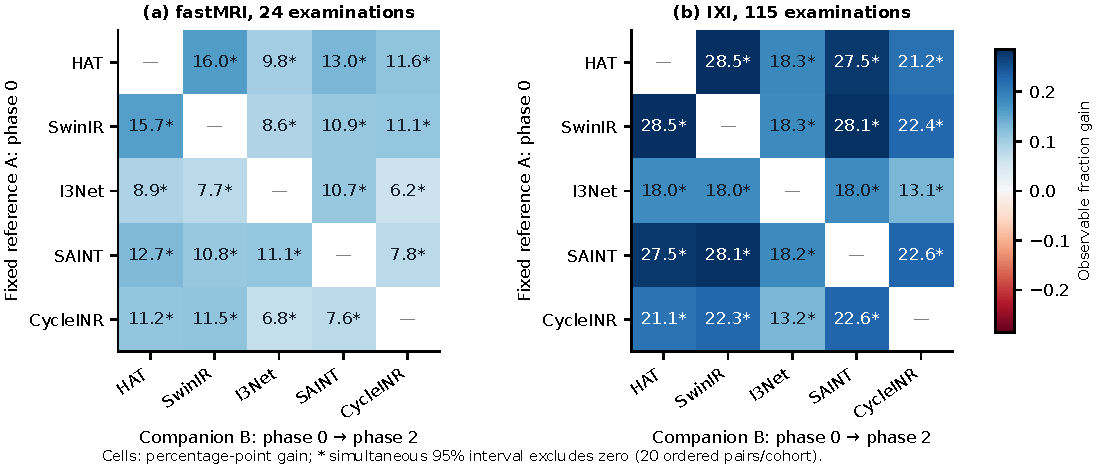
\includegraphics[width=.98\textwidth]{final_fig4_cross_architecture.pdf}
\caption{All cross-architecture measurement interventions, without TTA. Row A retains its phase-0 prediction; column B changes from phase 0 to phase 2 at the same target. Cells show mean observable-fraction gains in percentage points. Stars indicate simultaneous 95\% intervals excluding zero across all 20 ordered pairs per cohort. Diagonals are outside this cross-architecture design. The target-derived mask is identical across pairs and conditions.}
\label{fig:arch}
\end{figure*}

\paragraph{Post-hoc support and geometry checks.}
The same predictions retain all 20 positive simultaneous local intervals per cohort under acquired-anchor foreground union and full-image support; pair-effect ordering changes by at most one rank. Residue-1 and residue-3 estimates, their equal-weight average, and nearest-distance matching also retain all 20 positive intervals. However, mirror differences exclude zero for 8 fastMRI and 6 IXI pairs. The stricter four-neighbor, two-residue contract is feasible on IXI and NA on shallow fastMRI volumes. Thus balancing preserves the phenomenon but does not remove orientation/context effects. Joint examination bootstrap preserves pair dependence; leave-one-architecture-out family summaries stay positive. Complete post-hoc matrices and family intervals are in the supplement; the 20 pairs are not independent replications.

The examination-ranking boundary is substantial. Fixed-reference A-error ranking has 16 positive simultaneous intervals on IXI and four crossing zero (all with I3Net as companion); all 20 fastMRI intervals cross zero, including one negative point estimate. Condition-specific paired-error ranking has 20 positive intervals on IXI and none on fastMRI. Those endpoints are not interchangeable. The historical same-model five-architecture local effects and weaker ranking results remain in the supplement, together with the earlier analytical two-member ensemble contrast. Architecture diversity alone does not eliminate measurement dependence, and improved local observability does not imply universal ranking improvement.

\subsection{A fixed-context neural test of the local model}
At fixed nominal inputs, coupled perturbations reuse eight balanced fields on the common anchor; independent perturbations use their full $8\times8$ Cartesian product. Empirical marginals are identical. The matched finite-response covariance closes $\Delta\mathbb E D^2=-2\kappa$ numerically, which is an algebraic check. The substantive approximation test (Fig.~\ref{fig:influence}c) instead freezes the odd response at $\epsilon_0=.0025$ and predicts effects at .0025/.005/.01/.02 by $\epsilon^2$ scaling.

In the original HAT/SwinIR family, all eight model/amplitude mean effects are negative with simultaneous intervals below zero. Median relative approximation errors range from 1.9\% to 10.6\%; the worst individual error is 126.4\%, so the local trend is not a uniform approximation guarantee. Of 96 model/case/context combinations, 86 have aligned and 10 near-orthogonal reference sensitivities; none is opposing. All are retained. The experiment supports a conditional local sensitivity explanation, not the proposition's unobserved opposing-sensitivity branch or a claim that phase changes preserve bias/Jacobians. The same frozen validation on SAINT-style adds four negative mean intervals; median relative errors are 0.008--1.069\%, with a 3.199\% maximum. This non-transformer replication broadens the observed local trend without removing the original 126.4\% boundary or creating an opposing-sensitivity example.

\paragraph{Actionable scoring remains unresolved.}
The single acquired-only guard has no positive internal-evaluation cases and only two per pair on IXI; every IXI guard-minus-baseline simultaneous AP interval crosses zero. Its full negative evaluation and the earlier context-selection, jackknife and residualization failures remain in the supplement; no further score is searched.



\section{Discussion and Limitations}
MIRA separates replicated local observability loss, conditional influence/ranking support, and unestablished actionable reliability. Cross-architecture interventions address a TTA-only explanation; acquired-only probes address target-derived influence formation; fixed-context perturbations test a local approximation separately from its algebraic identity. None identifies arbitrary common bias without targets. Table~\ref{tab:continuous-big} shows all 13 bank entries; historical MIRA report cards in the supplement retain NA for fields absent from each design.

The principal limitations remain retrospective cohort reuse, incomplete historical selection chronology, residual phase-geometry/preprocessing changes, adapted implementations and limited independent patient counts. The full-bank acquired-only comparison covers 8 compatible implementations, including a linear control, on two brain cohorts. This does not erase historical knee/architecture failures or establish validity for the incompatible regular-grid models. MSValid and ReMIND supplied distinct patient-source, protocol-frozen HAT-to-SwinIR single-pair confirmations; the ReMIND design followed the MSValid result, and the later IXI-trained-weight MSValid pair reused the same patients. None replicated the architecture matrix or influence prediction. ReMIND DICOMs are labeled MPR and do not establish independently acquired original slices. Shared versus disjoint contexts change slice content, signed geometry and possibly normalization as well as overlap; post-result controls do not isolate a pure anchor-ID causal effect. Anonymous cross-dataset identifiers cannot prove patient non-overlap. Sampling intervals on old cohorts do not account for the full history of analysis selection. Local perturbations are not a validated clinical noise model. Neither lesion-level safety nor clinical outcomes were measured.

All 13 baseline models, 111 configurations and training-budget comparisons remain in the supplement, with adverse results intact. The new comparison evaluates 8 compatible implementations under one declared response protocol; interface-ineligible models remain in Table~\ref{tab:continuous-big}. They establish breadth of reconstruction evidence, not a new reconstruction method. Current-error adjustment weakens retrospective densification associations, Res-SRDiff retains an adverse boundary, and no clinical, prospective acquisition or non-MRI benefit is established.

\section{Conclusion}
Architectural diversity and evidence diversity are different axes. In these MRI interpolation experiments, different frozen architectures can inherit aligned error when they reuse the same measurements. Changing companion evidence reveals more of that error, including after support and residue-balancing checks, while residual orientation effects prevent a pure identity-only causal interpretation. Agreement among different networks therefore should not be treated as independent reliability evidence merely because their architectures differ.

MIRA makes this distinction testable through slice-context interventions, explicit information contracts and separate observability, influence and ranking fields. The prespecified MSValid pair, later frozen ReMIND source test and post-result same-patient IXI-weight pair strengthen the bounded observability claim at different evidence levels. Earlier numerically eligible response associations and fixed-context covariance experiments remain conditional mechanism evidence: SAINT mismatch sensitivity and the negative MSValid heldout prediction result preclude a portable influence score. None establishes universal ranking or calibrated uncertainty. MIRA measures when agreement loses observability, not whether an individual reconstruction is correct.

{\small\bibliographystyle{ieeenat_fullname}\bibliography{references}}
\end{document}
